\documentclass[tikz, border=4pt]{standalone}
\usepackage{tikz}
\usetikzlibrary{arrows.meta}
\begin{document}
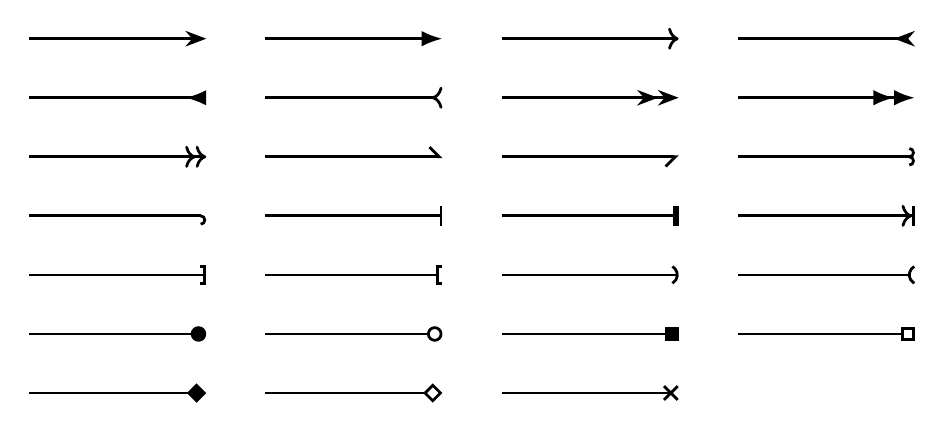
\begin{tikzpicture}[x=1cm, y=1cm]
  \draw[line width=1pt, -{Stealth}] (0,0) -- (2.25,0);
  \draw[line width=1pt, -{Latex}] (3,0) -- (5.25,0);
  \draw[line width=1pt, -{To}] (6,0) -- (8.25,0);
  \draw[line width=1pt, -{Stealth[reversed]}] (9,0) -- (11.25,0);
  \draw[line width=1pt, -{Latex[reversed]}] (0,-0.75) -- (2.25,-0.75);
  \draw[line width=1pt, -{To[reversed]}] (3,-0.75) -- (5.25,-0.75);
  \draw[line width=1pt, -{Stealth[] Stealth[]}] (6,-0.75) -- (8.25,-0.75);
  \draw[line width=1pt, -{Latex[] Latex[]}] (9,-0.75) -- (11.25,-0.75);
  \draw[line width=1pt, -{To[] To[]}] (0,-1.5) -- (2.25,-1.5);
  \draw[line width=1pt, -{Straight Barb[harpoon]}] (3,-1.5) -- (5.25,-1.5);
  \draw[line width=1pt, -{Straight Barb[harpoon, swap]}] (6,-1.5) -- (8.25,-1.5);
  \draw[line width=1pt, -{Hooks}] (9,-1.5) -- (11.25,-1.5);
  \draw[line width=1pt, -{Hooks[right]}] (0,-2.25) -- (2.25,-2.25);
  \draw[line width=1pt, -{Bar}] (3,-2.25) -- (5.25,-2.25);
  \draw[line width=1pt, -{Bar[] Bar[]}] (6,-2.25) -- (8.25,-2.25);
  \draw[line width=1pt, -{To[] Bar[]}] (9,-2.25) -- (11.25,-2.25);
  \draw[line width=1pt, -{Bracket}] (0,-3) -- (2.25,-3);
  \draw[line width=1pt, -{Bracket[reversed]}] (3,-3) -- (5.25,-3);
  \draw[line width=1pt, -{Parenthesis}] (6,-3) -- (8.25,-3);
  \draw[line width=1pt, -{Parenthesis[reversed]}] (9,-3) -- (11.25,-3);
  \draw[line width=1pt, -{Circle}] (0,-3.75) -- (2.25,-3.75);
  \draw[line width=1pt, -{Circle[open]}] (3,-3.75) -- (5.25,-3.75);
  \draw[line width=1pt, -{Square}] (6,-3.75) -- (8.25,-3.75);
  \draw[line width=1pt, -{Square[open]}] (9,-3.75) -- (11.25,-3.75);
  \draw[line width=1pt, -{Turned Square}] (0,-4.5) -- (2.25,-4.5);
  \draw[line width=1pt, -{Turned Square[open]}] (3,-4.5) -- (5.25,-4.5);
  \draw[line width=1pt, -{Rays[n=4]}] (6,-4.5) -- (8.25,-4.5);
\end{tikzpicture}
\end{document}
